\documentclass{../../presentation}

\title{PSE – Vorkurs Tag 3}
\author{Linus, Philipp, Tillmann, Tobias}
\institute{FIUS - Fachgruppe Informatik Universität Stuttgart}
\date{08.09.2025}

\makeatletter
\renewcommand{\lecture@pathprefix}[1]{../../logos/}
\makeatother

\usepackage{todonotes}
\setuptodonotes{inline}


\begin{document}

\begin{frame}
    \titlepage
\end{frame}

\begin{frame}
    \listoftodos
\end{frame}

\begin{frame}
    \frametitle{Recap Tag 2}
    \todo{am Anfang immer Vortages recap?}
\end{frame}

\begin{frame}[fragile]
    \frametitle{Angenommen \dots}
    \begin{itemize}
        \item Notendurchschnitt von zwei Studis berechnen
        \begin{minted}{java}
            // Melanie
            double m1 = 1.7, m2 = 2.3, m3 = 1.3;
            double melanieDurchschnitt = (m1 + m2 + m3) / 3;
            System.out.println("Melanies Schnitt: " + melanieDurchschnitt);

            // Paul
            double p1 = 4.0, p2 = 2.3, p3 = 3.3;
            double paulDurchschnitt = (p1 + p2 + p3) / 3;
            System.out.println("Pauls Schnitt: " + paulDurchschnitt);
        \end{minted}
        \begin{ausgabe}
            Melanies Schnitt: 1.7666666666666666 
        
            Pauls Schnitt: 3.1999999999999997
        \end{ausgabe}
    \end{itemize}
\end{frame}

\begin{frame}[fragile]
    \frametitle{Warum so nicht?!}
    \begin{itemize}
        \item\pause \textbf{Redundanz} \\
        Gleicher Code mehrfach – nur andere Zahlen

        \item\pause \textbf{Fehleranfällig} \\
        Ein Zahlendreher reicht, und das Ergebnis stimmt nicht

        \item\pause \textbf{Schlecht wartbar} \\
        Bei Änderungen muss alles händisch angepasst werden

        \item\pause \textbf{Nicht wiederverwendbar} \\
        Die Berechnung lässt sich nicht woanders nutzen

        \item\pause \textbf{Unübersichtlich} \\
        Zwischen vielen Zeilen geht die Logik unter
\end{itemize}
    \vspace{2em}
    \begin{minipage}{\textwidth}
	\centering
	\onslide\pause{\Huge $\rightarrow$~}%
	\onslide{\Large Funktionen retten uns vor Copy-Paste}
\end{minipage}
\end{frame}

\begin{frame}[fragile]
    \frametitle{Was sind eigentlich Funktionen?}
    \begin{itemize}
        \item  Möglichket Code auszulagern
        \item Syntax:
        \begin{minted}{java}   
Rückgabedatentyp Funktionsbezeichner(Datentyp Parametername,...){
        ...
        return Rückgabewert;
 }
        \end{minted}
        \item in unserem Fall:
        \begin{minted}{java}
        static void avg(String name, double note1, double note2, double note3) {
        double avg = (note1 + note2 + note3) / 3;
        System.out.println(name + "s Schnitt: " + avg);
            \end{minted}
        \item \textbf{Lösung:} Funktionen ermöglichen Wiederverwendung von Code!
    \end{itemize}
\end{frame}

%%ALT
\begin{frame}[fragile]
    \frametitle{Funktionen}
    \begin{itemize}
        \item Beim Programmieren benötigt man oft die gleiche Funktionalität an mehreren Stellen.
        \item Bisher musste man dafür den gleichen Code mehrfach schreiben.
        \item Das führt zu:
              \begin{itemize}
                  \item Viel Schreibarbeit
                  \item Fehleranfälligkeit (z.B. Tippfehler, unterschiedliche Änderungen)
              \end{itemize}
        \item \textbf{Lösung:} Funktionen ermöglichen Wiederverwendung von Code!
    \end{itemize}
\end{frame}

\begin{frame}
    \frametitle{Funktionen}
    \begin{itemize}
        \item Funktionen sind benannte Codeblöcke, die eine bestimmte Aufgabe erfüllen.
        \item Sie können Parameter entgegennehmen und einen Wert zurückgeben.
        \item Beispiel: Die PSE-Vorkurs Orgas haben sich ordentlich einen hinter die Rüstung gerömert und wollen jeweils wissen, wie viel Promille sie haben.
    \end{itemize}
\end{frame}

\begin{frame}[fragile]
    \frametitle{Funktionen}
    Mithilfe von Funktionen können wir eine oder mehrere Codezeilen auslagern und an verschiedenen Stellen im Code aufrufen.
    \begin{itemize}
        \item Funktionen haben \textbf{Parameter} (= Werte, die der Funktion übergeben werden).
        \item Funktionen besitzen einen \textbf{Rückgabewert}, ähnlich wie mathematische Funktionen, z.\,B.\ $f(x) = x^2$.
        \item Der Rückgabewert wird mit \texttt{return} zurückgegeben; danach wird die Funktion abgebrochen.
    \end{itemize}
    \begin{minted}{java}
Rückgabedatentyp Funktionsbezeichner(Datentyp1 Parametername1, ...) {
    ...
    return Rückgabewert;
}
\end{minted}
\end{frame}

\begin{frame}[fragile]
    \frametitle{Funktionen}
    \begin{itemize}
        \item man kann so viele Parameter angeben, wie man will
        \item Parameter können verschiedene Datentypen haben
        \item Rückgabewert kann auch \texttt{void} sein, wenn die Funktion keinen Wert zurückgibt
    \end{itemize}
    \begin{minted}{java}
    void begruessen(String name) {
        System.out.println("Hallo, " + name + "!");
    }
    \end{minted}
\end{frame}
%%


\begin{frame}[plain]
    \centering
    {\Huge\bfseries{Code together}}
    \begin{block}{}
        \[
            \text{Promille} \approx \frac{\text{Alkohol in Gramm}}{\text{Körpergewicht in kg} \times 0{,}65}
        \]
        \[
            \text{Alkohol in Gramm} = \text{Getränkemenge in Liter} \times \text{Vol\%} \times 8
        \]
    \end{block}
\end{frame}

\begin{frame}[fragile]
    \frametitle{Main-Funktion}
    \begin{itemize}
        \item Die \texttt{main}-Funktion ist der Einstiegspunkt für jedes Java-Programm.
        \item Sie wird automatisch aufgerufen, wenn das Programm gestartet wird.
        \item Die \texttt{main}-Funktion muss immer so aussehen:
              \begin{minted}{java}
public static void main(String[] args) {
    // Hier beginnt das Programm
}
\end{minted}
    \end{itemize}
\end{frame}

\begin{frame}[fragile]
    \frametitle{Basic Scopes}
    \begin{itemize}
        \item Variablen, die \textbf{in einer Funktion} definiert sind, können nur in dieser Funktion verwendet werden.
        \item Variablen, die \textbf{außerhalb einer Funktion} definiert sind, können auch in der Funktion verwendet werden.
        \item Bei korrekter Einrückung gilt: Variablen sind in den \textbf{kleineren Ebenen} sichtbar, aber nicht in den darüberliegenden.
        \item Das gilt auch für Schleifen, \texttt{if}-Blöcke usw.
    \end{itemize}
\end{frame}

\begin{frame}[fragile]
    \frametitle{Basic Scopes}
    
\includegraphics[width=1\linewidth]{img/scopesmemehoriz.png}
\end{frame}


\begin{frame}[fragile]
    \frametitle{Arrays}
    Mit \textbf{Arrays} kann eine Sammlung von Werten des gleichen Datentyps gespeichert werden.
    \begin{itemize}
        \item Alle Elemente in einem Array müssen den gleichen Datentyp haben (z.\,B.\ \texttt{int}, \texttt{double}, \texttt{String}).
        \item Ein Array hat eine feste Länge, die beim Erstellen festgelegt wird.
        \item Die Elemente im Array sind geordnet und über einen \textbf{Index} erreichbar.
    \end{itemize}
    \begin{minted}{java}
        Datentyp[] Bezeichner = new Datentyp[ArrayLänge];
    \end{minted}
\end{frame}

\begin{frame}[fragile]
    \frametitle{Zugriff auf Elemente eines Arrays}
    \begin{itemize}
        \item Jedes Element hat eine Nummer (index)
        \item Wir können über den Index auf die Elemente zugreifen
    \end{itemize}
    \begin{columns}
        \column{0.5\linewidth}
        \begin{minted}{java}
            int[] array = new int[5];
            array[0] = 6;
            array[2] = 9;
        \end{minted}

        \column{0.5\linewidth}
        \begin{center}
            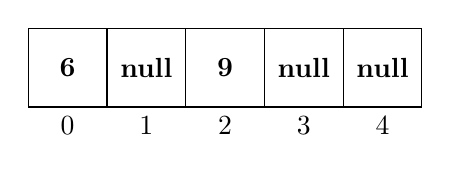
\begin{tikzpicture}
                \foreach \x in {0,1,...,4} {
                        \draw (\x,0) rectangle coordinate(c\x) (\x+1, 1);
                        \node[below] at (\x+0.5, 0) {\x};
                    }
                \node at (c0) {\bf 6};
                \node at (c1) {\bf null};
                \node at (c2) {\bf 9};
                \node at (c3) {\bf null};
                \node at (c4) {\bf null};
            \end{tikzpicture}
        \end{center}
    \end{columns}

    \vspace{0.5cm}

    \begin{itemize}
        \item Die Array-Variable speichert die Länge das arrays: \mintinline{java}{array.length}
        \item Der höchste Index ist immer \mintinline{java}{array.length - 1}
    \end{itemize}
\end{frame}

\begin{frame}[fragile]
    \frametitle{Arrays}
    Wir können Arrays auch direkt mit Werten initialisieren
    \begin{minted}{java}
    String[] grillSachen = {"würstchen", "steak", 
                            "grillkäse", "maiskolben"};
    \end{minted}
    Und wir können sie auch mit einer Schleife durchlaufen:
    \begin{minted}{java}
    System.out.println(grillSachen[1]);
    for (int i = 0; i < grillSachen.length; i++) {
        System.out.println(grillSachen[i]);
    }
    \end{minted}
\end{frame}

\end{document}
